\chapter{Evaluation}
All is outline:

\section{Presence notifications}
I have \code{roster/alice.xml}, \code{roster/bob.xml}, \code{roster/caroll.xml}. I have evidence that their consecutive connections produce the correct presence-notification patterns in accordance with their subscriptions to each other, though only in one of the six orders of connection. [should I bother being exhaustive with this?]

\section{Roster management}
I have evidence that in the aforementioned connections the clients receive their rosters as expected. The lack of CRUD operations means there is little else to do.

\section{Handshake; connect / disconnect}
I have screenshot and logs collectively showing the following:
\begin{itemize}
  \item Working handshake between Psi and server, plus appropriate \code{feature-not-implemented} response to the non-core features Psi requests
  \item Conversation between Bob and Caroll via the Psi messaging interface and the \code{Client} module respectively
\end{itemize}

\section{Messaging}
\subsection{Throughput}
My primary aim was to see how throughput of message delivery was affected by the number of connected clients. To do this, I somehow needed a throughput figure for different client counts. Thus, I investigated how throughput varied over time for different client counts, hoping to see the value stabilise.

To keep the client controller simple, I adopted following model: $n$ clients send a fixed message to $n$ other clients, as fast as possible, until the program is manually terminated. To begin with, I used a 445-byte text string which, when wrapped in the XML \code{message} element, ran over the 512-byte size of the parsing buffers.

The server samples its throughput at regular intervals and outputs the values. It does this by keeping track of how many messages it delivered in the last 5 seconds; this message count is then divided by the actual time elapsed, which stays close to 5 seconds.

\subsubsection{Throughput over time}
The characteristic in Figure~\ref{fig:5n5} shows a normal characteristic which stabilises.
\begin{figure}
  \centering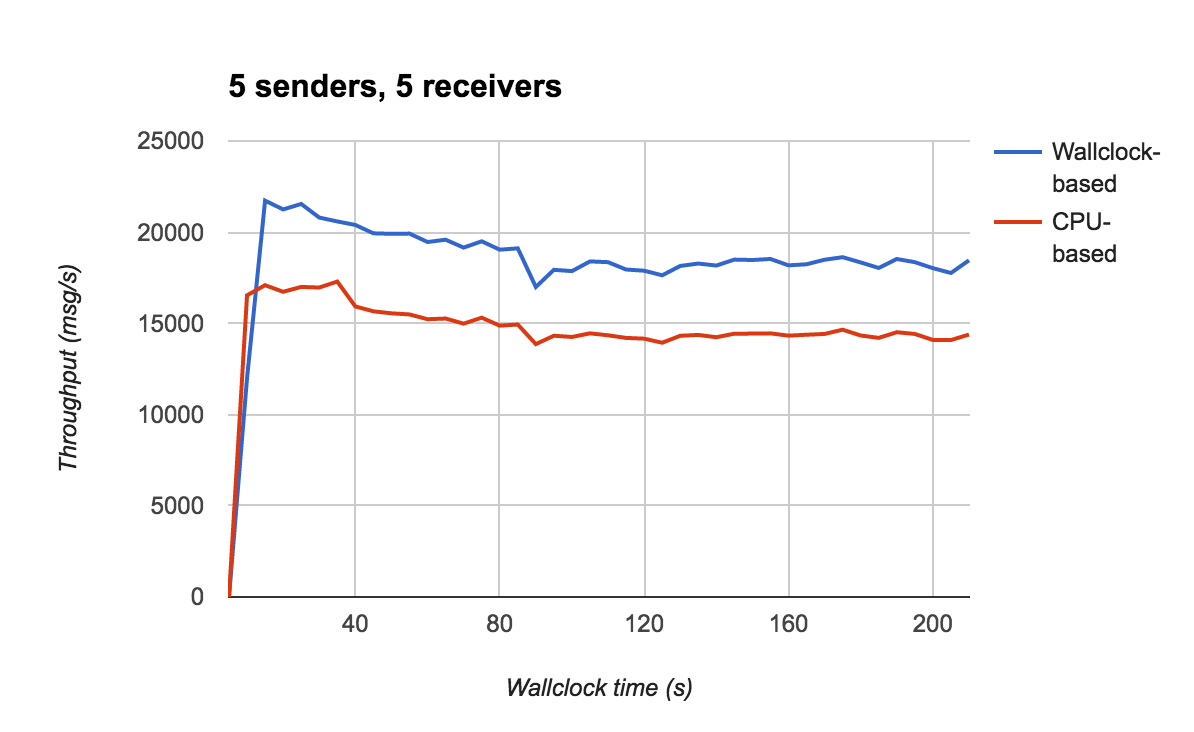
\includegraphics[width=\textwidth]{../transcripts/lipsum/5n5/graph.png}
  \caption{5 send-receive pairs.}
  \label{fig:5n5}
\end{figure}

In Figure~\ref{fig:10n10}, at 10 client pairs, there is an odd dip at around $t=300s$.
\begin{figure}
  \centering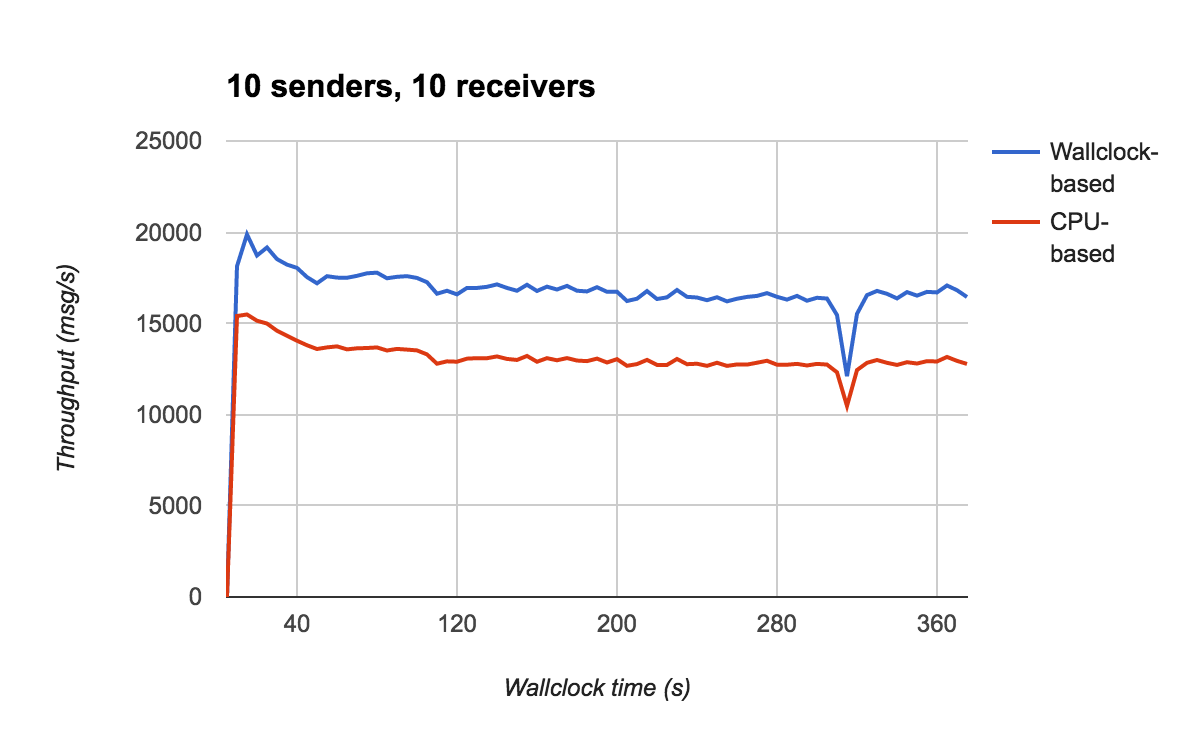
\includegraphics[width=\textwidth]{../transcripts/lipsum/10n10/graph.png}
  \caption{10 send-receive pairs.}
  \label{fig:10n10}
\end{figure}

From 15 to 20 (Figure~\ref{fig:15n20}), we see much more chaotic behaviour from $t=300s$ that does not seem to stabilise:
\begin{figure}
  \centering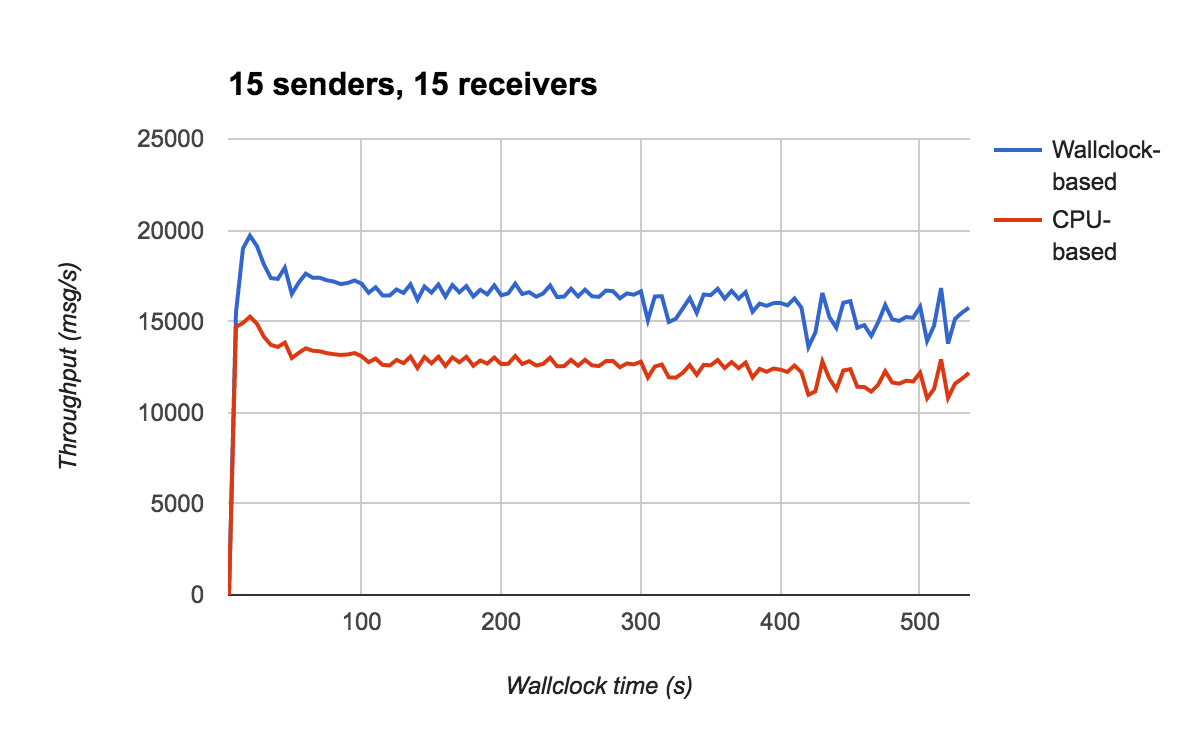
\includegraphics[width=\textwidth]{../transcripts/lipsum/15n15/graph.png}

  \centering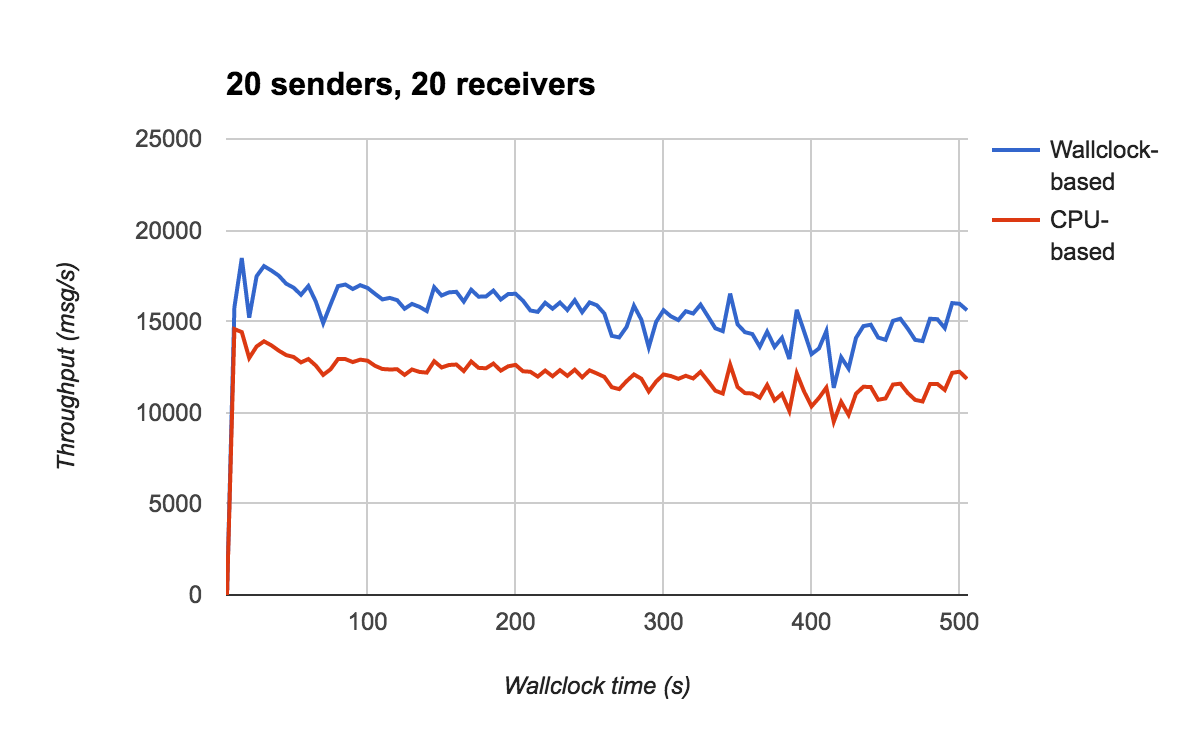
\includegraphics[width=\textwidth]{../transcripts/lipsum/20n20/graph.png}
  \caption{20 send-receive pairs.}
  \label{fig:15n20}
\end{figure}

Stabilisation begins to return at 25 and beyond in Figure~\ref{fig:lots}. (Supposed to show 25-60)
\begin{figure}
  \centering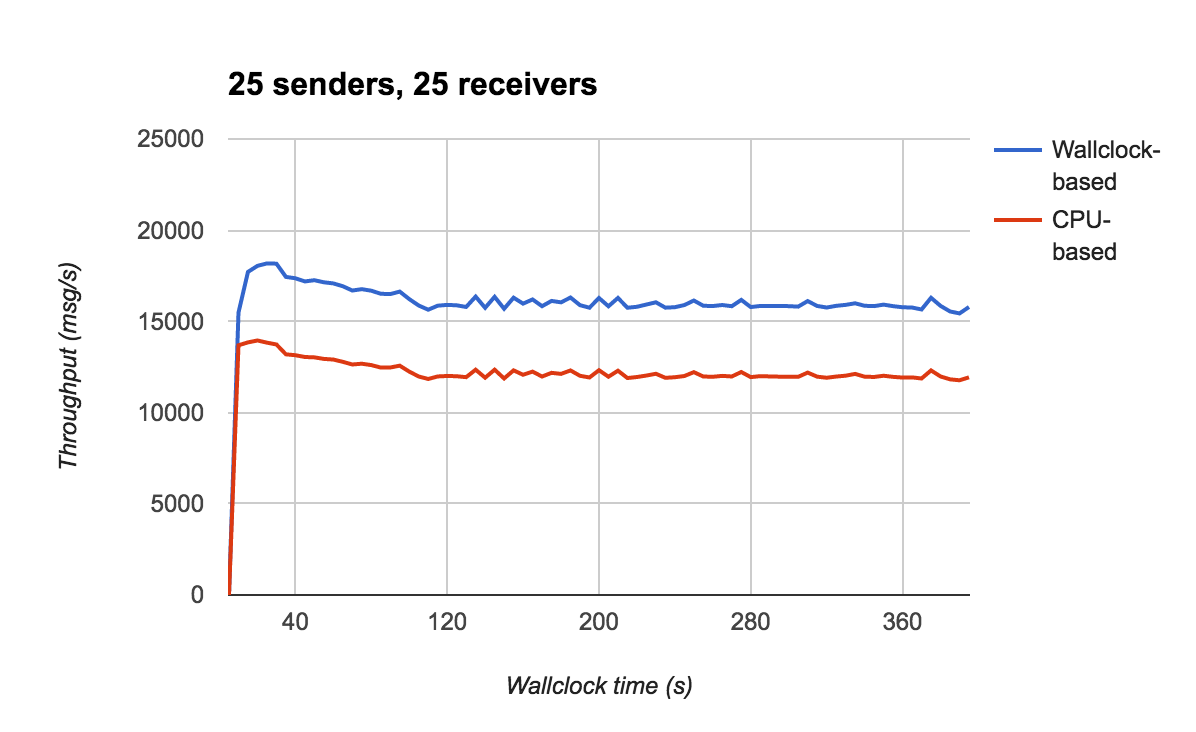
\includegraphics[width=\textwidth]{../transcripts/lipsum/25n25/graph.png}

  \centering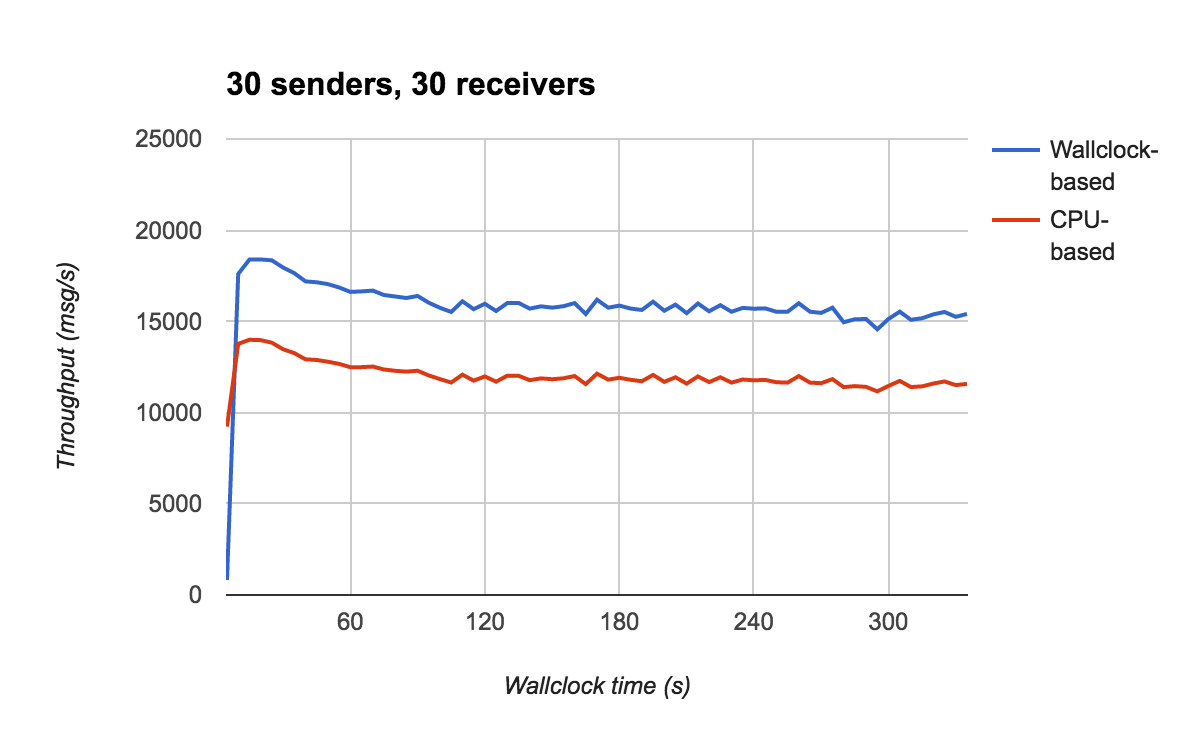
\includegraphics[width=\textwidth]{../transcripts/lipsum/30n30/graph.png}
  \caption{30 send-receive pairs.}
  \label{fig:lots}
\end{figure}
\begin{figure}
  \centering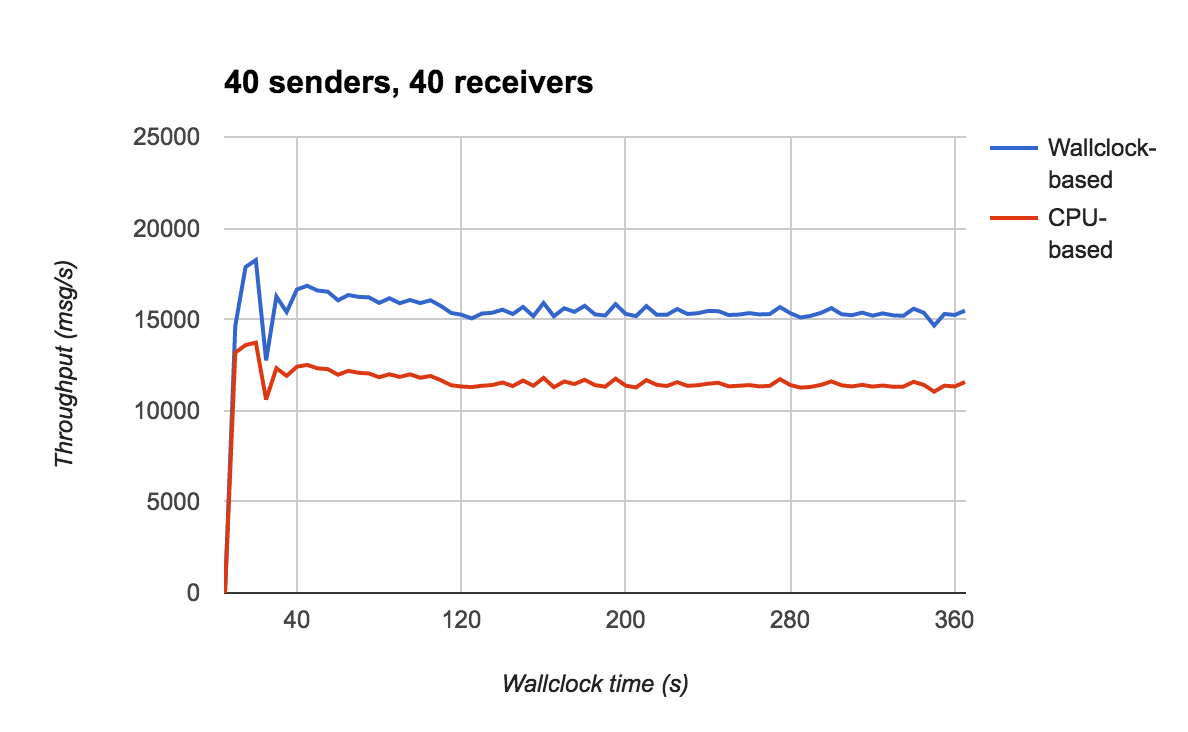
\includegraphics[width=\textwidth]{../transcripts/lipsum/40n40/graph.png}
\end{figure}
\begin{figure}
  \centering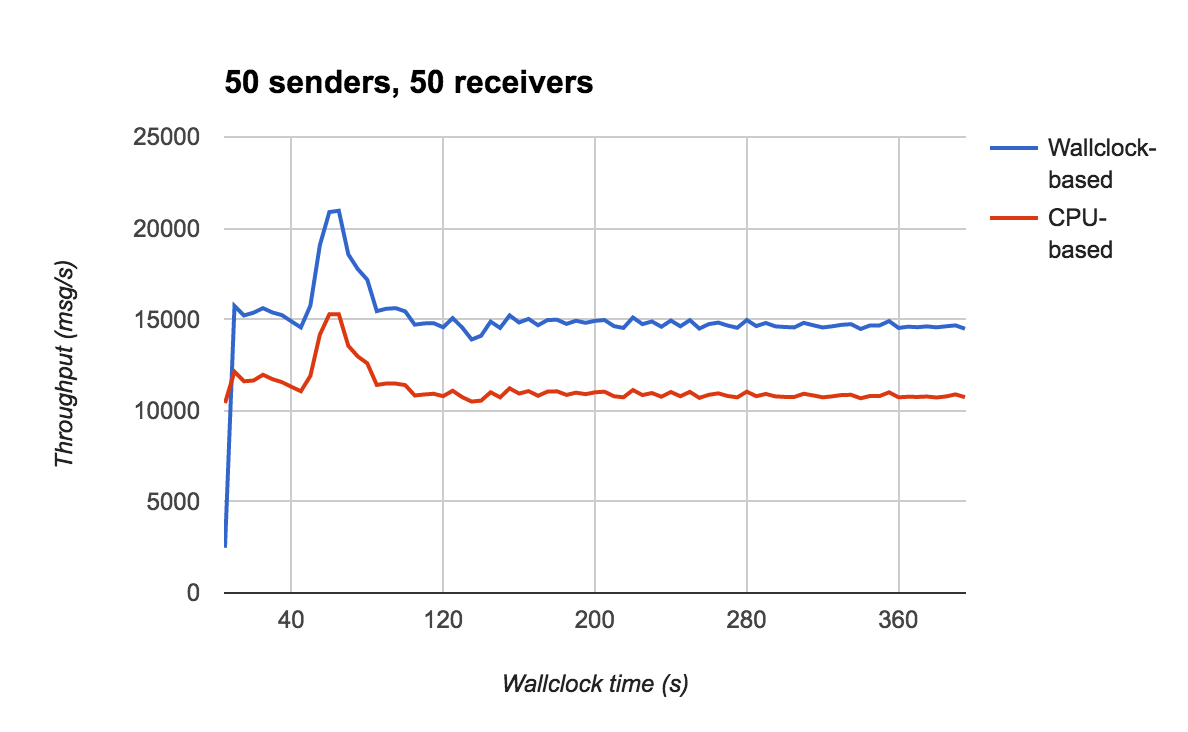
\includegraphics[width=\textwidth]{../transcripts/lipsum/50n50/graph.png}
\end{figure}
\begin{figure}
  \centering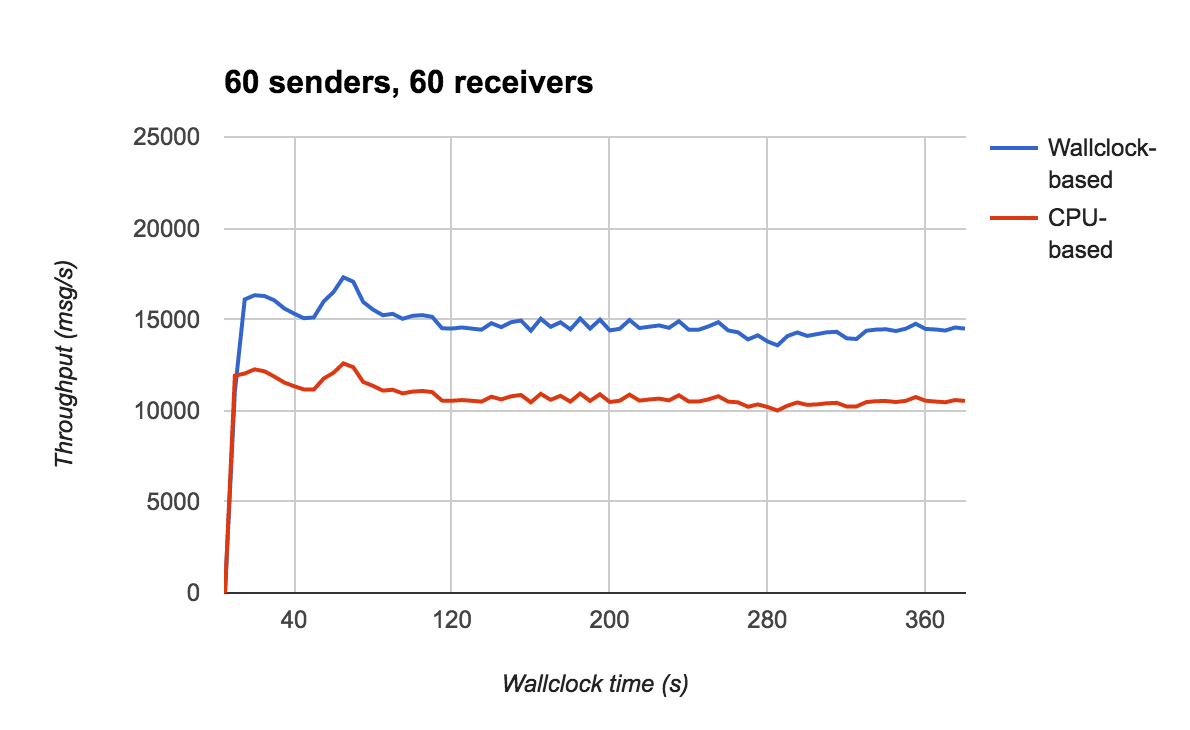
\includegraphics[width=\textwidth]{../transcripts/lipsum/60n60/graph.png}
\end{figure}

I took the average of throughput samples in the stable-looking regions (or, for the chaotic graphs, the relatively stable-looking regions) and took the values as the ``operating throughputs'' of my server for these parameters. From this I obtained the indication of operating throughput as a function of client load shown in Figure~\ref{fig:summary}.

\begin{figure}
  \centering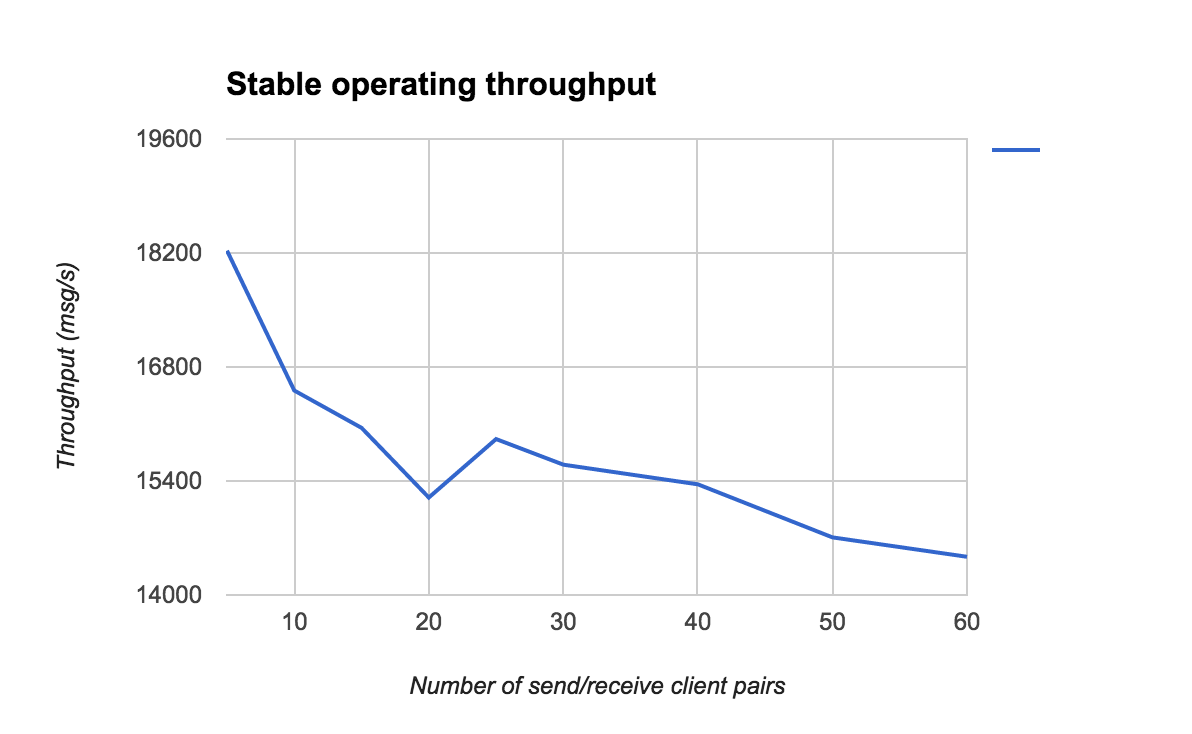
\includegraphics[width=\textwidth]{../transcripts/lipsum/throughp_clients.png}
  \caption{Effect of client load on operating throughput.}
  \label{fig:summary}
\end{figure}
